\documentclass[12pt, letterpaper]{article}
\usepackage[utf8]{inputenc}
\usepackage{amsmath}
\usepackage{amssymb}
\usepackage{amsfonts}
\usepackage{tcolorbox}
\usepackage{graphicx}
\usepackage{hyperref}
\usepackage{listings}
\usepackage{setspace}
\hypersetup{
    colorlinks,
    citecolor=black,
    filecolor=black,
    linkcolor=black,
    urlcolor=black
}
\lstset{
  language     = C,
  basicstyle   = \ttfamily,
  commentstyle = \color{blue},
  stringstyle  = \color{green!70!black},
  stringstyle  = \color{gray},
  columns      = fullflexible,
  numbers      = left,
  numberstyle  = \scriptsize\sffamily\color{gray},
  showstringspaces = false,
  float,
}
\graphicspath{{./images/}}

\newcommand*{\QEDB}{\null\nobreak\hfill\ensuremath{\square}}%
\newcommand\tab[1][1cm]{\hspace*{#1}}
\newcommand\tabd[1][0.3cm]{\hspace*{#1}}

\title{
        \Huge{Especificação da Linguagem \\[10mm]}
        \centering 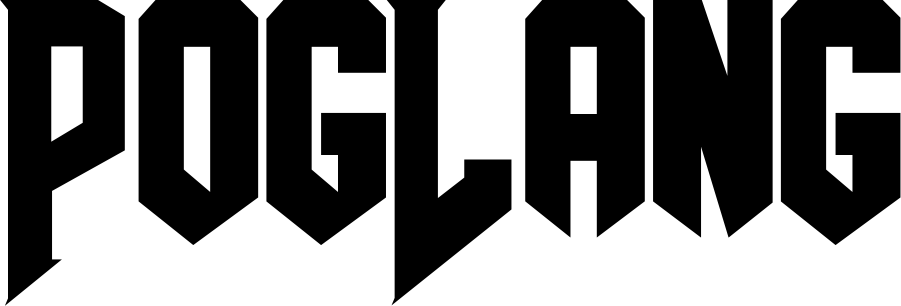
\includegraphics[scale=0.25]{PogLang}
}

\author{}
\date{}


\begin{document}

\maketitle
\textit{
        \centering\LARGE{
                Jonas Edward Tashiro\\ 
                Luan Lopes Barbosa de Almeida\\ 
                Rafael Melloni Chacon Arnone\\ 
                Mateus Assalti Santana\\
        }
}

%\begin{center}
%\hypertarget{loretta}{}
%\end{center}

\newpage
\tableofcontents

\newpage
\section{Introdução}
\tab\large PogLang é uma linguagem procedural que possui inspiração nas linguagens C, GO e Rust; é fortemente
tipada, estaticamente tipada e não possui um garbage colector (diferente de GO).\\[1.0mm]
\tab O objetivo do PogLang é ser uma linguagem educativa, mostrando o processo de criação de um Compilador com 
capacidade de compilar tanto para processadores x86 quanto para o bytecode do WebAssembly.\\[1.0mm]

\section{Variáveis e Operadores}
\subsection{Declarações e Tipos}
\tab Na linguagem PogLang todas as variáveis devem ser declaradas antes de serem usadas, isto é, o tipo 
deve indicado de forma explicita junto ao nome da variável, sendo que o tipo é escrito primeiro seguido 
do nome da variável. \\[1.0mm]
\tab Também é possível declarar várias variáveis do mesmo tipo, na qual, após escrevermos o tipo da variável  
colocamos uma lista com o nome das variáveis separadas por ','. \\[1.0mm]

\begin{spacing}{1.5}
\end{spacing}

\begin{lstlisting}[caption=Exemplo declaração de variáveis]
int pog;
int x, y, z;
\end{lstlisting}

\begin{spacing}{1.5}
\end{spacing}

\tab Outra forma de declararmos uma variável é através da palavra-chave let, na qual inicializamos uma variável 
com um valor definido. Neste caso não é necessário declarar o tipo da variável, pois este é inferido a partir do 
literal a direita do símbolo de igualdade '='. 

\begin{spacing}{1.5}
\end{spacing}

\begin{lstlisting}[caption=Exemplo inicialização com palavra-chave let]
let x = 2; //declara e inicia uma variavel do tipo int
let f = 3.14f  //declara e inicia uma variavel do tipo float
let a = [1,2,3] //declara e inicia um array do tipo int
\end{lstlisting}

\begin{spacing}{1.5}
\end{spacing}

\tab Na questão do tipo de variáveis, a linguagem PogLang possui os seguintes tipos apresentados na tabela abaixo:

\begin{spacing}{1.5}
\end{spacing}

\begin{center}
\begin{tabular}{c c c}
Type & Bytes & Intervalo \\
char & 8 & 0 até 255 \\
int & 32 & –32,767 até 32,767 \\
uint & 32 & 0 até 65,535 \\
float & 32 & $–3.4 \cdot 10^{38}$ até $+3.4 \cdot 10^{38}$ \\
double & 64 & $–1.8 \cdot 10^{308}$ até $+1.8 \cdot 10^{308}$ \\
bool & 32 & - \\
\end{tabular}
\end{center}

\begin{spacing}{1.5}
\end{spacing}

\tab A linguagem PogLang possui vários tipos de operadores, sendo que estes podem ser divididos nas seguintes classes: 
aritméticos, relacionais e lógicos, sendo que, o único operador que fica separado destas classes e o operador de
atribuição e é este que analisamos em seguida.


\subsection{Operador: Atribuição}
\tab O operador de atribuição e uma relação binaria que copia o valor de uma expressão no local do operando da direita
para uma variável na posição de operando esquerdo, sendo que ambos os operandos necessitam ser do mesmo tipo.\\[1.0mm]
\tab Portanto a linguagem PogLang segue a mesma definição de atribuição da linguagem C.


\begin{spacing}{1.5}
\end{spacing}

\begin{lstlisting}[caption=Exemplos de Atribuição]
let y = 2;
int x;
x = (3 + 5) * y;
\end{lstlisting}

\begin{spacing}{1.5}
\end{spacing}

\subsection{Operadores Aritméticos}
\tab A tabela a seguir mostra os operadores aritméticos e seus efeitos:  

\begin{spacing}{1.5}
\end{spacing}

\begin{center}
\begin{tabular}{c c}
Operador & Ação \\
- & Subtração, menos unário \\
+ & Adição \\
* & Multiplição \\
/ & Divisão \\
\% & Resto de Divisão \\
\end{tabular}
\end{center}

\begin{spacing}{1.5}
\end{spacing}

\subsection{Operadores Relacionais}
\tab A tabela a seguir mostra os operadores relacionais e seus efeitos:  

\begin{center}
\begin{tabular}{c c}
Operador & Ação \\
\textgreater & Maior que \\
\textgreater= & Maior que ou igual ($\geq$) \\
\textless & Menor que \\
\textless= & Menor que ou igual ($\leq$) \\
= & Igual \\
!= & Não igual($\neq$) \\
\end{tabular}
\end{center}

\begin{spacing}{1.5}
\end{spacing}

\subsection{Operadores Lógicos}
\tab A tabela a seguir mostra os operadores lógicos e seus efeitos:  

\begin{spacing}{1.5}
\end{spacing}

\begin{center}
\begin{tabular}{c c}
Operador & Ação \\
\&\& & AND \\
$||$ & OR \\
! & NOT \\
\end{tabular}
\end{center}

\begin{spacing}{1.5}
\end{spacing}

\subsection{Precedência de Operadores}
\tab Uma parte importante sobre operadores e a questão de precedência, na qual os certos operadores
tem prioridade ao serem encontrados em uma expressão, i.e., são realizados primeiro. A questão da 
precedência, se não entendida, pode gerar expressões ambíguas, portanto a tabela a seguir e fornecida.
  

\begin{spacing}{1.5}
\end{spacing}

\begin{center}
\begin{tabular}{c c}
Maior & () [] \\
 & ! \\
 & * / \% \\
 & + - \\
 & \textless \textless= \textgreater \textgreater= \\
 & == != \\
 & \&\& \\
Menor & $||$ \\
\end{tabular}
\end{center}

\begin{spacing}{1.5}
\end{spacing}

\section{Literais}

\tab Literais são valores constantes para certos tipos de dado que são representados por certas cadeias 
de caracteres.
\\[1.0mm]

\tabd Há seis literais no PogLang:

\begin{center}
        \begin{itemize}
                \item Integer literal
                \item Float literal
                \item Double literal
                \item Character literal
                \item String literal
                \item Boolean literal
        \end{itemize}
\end{center}

\begin{spacing}{1.5}
\end{spacing}

\tabd O \textit{Integer literal} representa apenas valores inteiros, sendo que este
é escrito na base decimal. Por exemplo, 45, 69, 420, etc.\\[1.0mm]
\tab O \textit{Float literal} representa números reis. Sua representação e particionada em duas partes, 
separadas pelo caractere '.', a parte inteira e a parte fracionada. Do mesmo modo que representamos
\textit{Integer literal} em base decimal, fazemos o mesmo \textit{Float literal} com a adição de um sufixo que 
permite a diferenciação de um \textit{Double literal}, que segue as mesmas especificações.

\begin{itemize}
        \item f: especifica o literal como do tipo float. Por exemplo, $4.0f$, $32.7f$, etc.
        \item lf: especifica o literal como do tipo double. Por exmplo, $1024.0lf$, $128.89lf$, etc.
\end{itemize}

\begin{spacing}{1.5}
\end{spacing}

\tabd O \textit{Character literal} é apenas um caractere delimitado dentro de aspas simples. Por exmplo, 'a',
'b', etc.\\[1.0mm]
\tab O \textit{String literal} é uma cadeia de caracteres delimitada dentro de aspas dulplas. Por exemplo,
"Hello", "Fuba", etc.\\[1.0mm]
\tab O \textit{Boolean literal} possui apenas dois valores, true e false.

\section{Instruções de Repetição}
\tab Em uma linguagem de programação as instruções de repetição controlam 
a quantidade de vezes que um bloco será executado baseado em uma condição,
essas instruções são também chamadas de loops sendo alguns exemplos as
instruções de while e for e do-while.

\begin{spacing}{1.5}
\end{spacing}

\begin{lstlisting}[caption=Forma geral do while] 
while expression
{
    statements
}
\end{lstlisting}

\begin{lstlisting}[caption=Exemplo while]
int i = 0;
while i < 5
{
    print(i);
    i = i + 1;
}
\end{lstlisting}

\begin{spacing}{1.5}
\end{spacing}

\tab Neste exemplo a saída no terminal possui números de 0 até 4.\\[1.0mm]
\tab A instrução while representa um loop onde, enquanto a expressão for 
verdadeira nos executamos o statement.

\begin{spacing}{1.5}
\end{spacing}

\begin{lstlisting}[caption=Forma geral do for]
for i in 0..n
{
    statements
}
\end{lstlisting}

Um exemplo dessa instrução seria:

\begin{lstlisting}[caption=Exemplo for]
for i in 0..5 
{
    print(i)
}
\end{lstlisting}

\begin{spacing}{1.5}
\end{spacing}

\tab Neste exemplo a saída no terminal e a mesma do Exemplo while.\\[1.0mm]
\tab A instrução for representa um loop cujo funcionamento pode ser compreendido 
atraves da frase "para i de um 0 até n-1 execute um determinado bloco".

\begin{spacing}{1.5}
\end{spacing}

\begin{lstlisting}[caption=Forma geral do do-while]
do
{
    statements
} while expression;
\end{lstlisting}

\begin{lstlisting}[caption=Exemplos do-while]
int i = 0;
do
{
    print(i);
    i = i + 1;
} while i < 5;
\end{lstlisting}

\begin{spacing}{1.5}
\end{spacing}

\tab A instrução do-while representa um loop que já começa executando 
determinado statement e verifica a expressão para realizar a execução do
statement novamente após já ter executado ele uma vez.

\section{Instrucoes de Controle}
\tab Em uma linguagem de programação as instruções de controle controlam a 
ordem de execução das instruções com base em uma condição,\\[1.0mm]
\tab Na linguagem Poglang um ";" indica o final de uma expressão, nessa linguagem
as chaves "\{" e "\}" são utilizadas para agrupar declarações e expressões
em um bloco, uma observação e que não precisamos adicionar ";" após um "\}" 
para indicar o final do bloco.\\[1.0mm]
\tab A instrução if-else e utilizada para representar uma decisão, podendo ser
representada através deste trecho, na qual o else e opcional:

\begin{spacing}{1.5}
\end{spacing}

\begin{lstlisting}[caption=Forma geral if-else]
if expression {
   statement1
} else {
   statement2
}
\end{lstlisting}

\begin{spacing}{1.5}
\end{spacing}

\tab Quando avaliada a expression (tipo booleano) for avaliada, se for verdadeira (true) o statement1 
e executado, caso contrário se o else existir executamos o statement2.

\begin{spacing}{1.5}
\end{spacing}

\begin{lstlisting}[caption=Forma Geral de múltiplos if-else]
if expression {
    statement
} else if expression {
    statement
} else {
    statement
}
\end{lstlisting}

\begin{spacing}{1.5}
\end{spacing}
 
\tab Outro constructo suportado pela Poglang e o else-if que representa uma 
decisão com múltiplos caminhos, as expressões são avaliadas em ordem, se
essa expressão for verdadeira então o statement relacionado a ela será 
executado terminando com a cadeia de decisão, nesse caso podemos utilizar 
o else para representar todas as outras alternativas.\\[1.0mm]

\tab Para podermos ilustrar um exemplo utilizando instruções de controle vamos 
demonstrar o exemplo de busca binaria, em que o array itens está ordenado
e x representa o item que desejamos encontrar.

\begin{spacing}{1.5}
\end{spacing}

\begin{lstlisting}[caption=Exemplo if-else]
fn binsearch(int x, int[] items) -> int 
{
        int low, high, mid;
        low = 0;
        high = items.len() - 1;
        while low <= high
        {
                mid = (low + high)/2;
                if x < items[mid] {
                        high = mid + 1;
                } else if x > items[mid] {
                        low = mid + 1;
                } else {
                        return mid;
                }
        }
        return -1;
}
\end{lstlisting}

\begin{spacing}{1.5}
\end{spacing}

\section{Arrays}
\tab Arrays em uma linguagem de programação são espaços contíguos na memoria
do computador, na linguagem Poglang temos um diferencial da linguagem C, 
o armazenamento do tamanho do array, facilitando o 
uso arrays.\\[1.0mm]

\tab Podemos instanciar um array através da seguinte expressão:

\begin{spacing}{1.5}
\end{spacing}

\begin{lstlisting}[caption=Forma geral do array]
type[size] name;
\end{lstlisting}

\begin{spacing}{1.5}
\end{spacing}

\tab Em que type representa o tipo da variável que será armazenado em nosso espaço
de memória contiguo e size o tamanho desse espaço e finalmente name que representa 
o nome da nossa variável.\\[1.0mm]

\begin{spacing}{1.5}
\end{spacing}

\begin{lstlisting}[caption=Exemplo de declaração de um array]
int[4] array;
\end{lstlisting}

\begin{spacing}{1.5}
\end{spacing}

\tab Podemos utilizar o método len no nosso array para descobrir seu tamanho,
nesse caso array.len() resultaria em 4.\\[1.0mm]
\tab O exemplo abaixo mostra como utilizar o método len para mostrarmos na tela
números de 0 até 3:

\begin{spacing}{1.5}
\end{spacing}

\begin{lstlisting}[caption=Exemplo uso do for para um array]
int[4] array;
for i in 0..array.len() 
{
    print(i);
}
\end{lstlisting}

\begin{spacing}{1.5}
\end{spacing}

\tab Podemos inicializar um array com itens através da sintaxe, na qual esses itens
precisam ser do mesmo tipo de separados por vírgula:

\begin{spacing}{1.5}
\end{spacing}

\begin{lstlisting}[caption=Exemplo inicialização de array com let]
let nome = [item1, item2,...itemN];
\end{lstlisting}

\begin{spacing}{1.5}
\end{spacing}

\tab Podemos, ainda assim, determinar o tamanho do array mesmo que este não tenha sido declarado
de maneira explicita ao utilizar a inicialização acima\\[1.0mm]

\begin{spacing}{1.5}
\end{spacing}

\begin{lstlisting}[caption=Exemplo do .len()]
let array = [1, 2, 3, 4];
for i in 0..array.len() 
{
    print(array[i]);
}
\end{lstlisting}

\begin{spacing}{1.5}
\end{spacing}

\section{String}
\tab Na linguagem Poglang as strings são uma cadeia de caracteres guardados em um array de chars.
Diferente da linguagem C não utilizamos um caractere para delimitar o fim da string,
uma vez que, arrays conseguem utilizar o método len para retornar o seu tamanho.\\[1.0mm]
\tab O exemplo abaixo demonstra o uso de string para mostrar na tela a
palavra "pog":

\begin{spacing}{1.5}
\end{spacing}

\begin{lstlisting}[caption=Exemplo string]
char[3] name = ['p', 'o', 'g'];
for i in 0..name.len()
{
    print(name[i]);
}
\end{lstlisting}

\begin{spacing}{1.5}
\end{spacing}

\section{Funções}
\tab Funções provem um modo conveniente de encapsular e modularizar alguma computação, 
na linguagem PogLang este importante conceito se inspirou nas linguagens Rust e GO\\[1.0mm]
\tab O próximo exemplo demostra um exemplo de uma função modelando a ideia matemática 
dá função de exponenciação em números inteiros.

\begin{spacing}{1.5}
\end{spacing}

\begin{lstlisting}[caption=Exemplo função power]
fn power(int m, int n) -> int
{
  for i in 1..=n
  {
    m = m * m;
  }
  return m;
}
\end{lstlisting}

\begin{spacing}{1.5}
\end{spacing}

\tabd Na primeira linha, a função é identificada pela palavra reservada fn e ao lado
temos o nome da função, nomes e tipos dos parâmetros e após a flecha "-\textgreater"
o tipo do retorno da função.\\[1.0mm]
\tab Os parâmetros são colocados entre os parênteses e são separados pelo símbolo ',',
sendo que, estas variáveis são locais a função, i.e., não são visíveis para demais 
regiões do código, somente no escopo da função.\\[1.0mm]
\tab O valor que power calcular é retornado através da palavra-reservada return, na qual, 
o retorno de uma função pode ser qualquer um dos tipos definidos na linguagem e 
vazio através da palavra reservada void.\\[1.0mm]
\tab Para uma definição mais geral de função, estas tem a seguinte forma:

\begin{spacing}{1.5}
\end{spacing}

\begin{lstlisting}[caption=Forma geral de funções]
fn funtion-name(parameter declarations) -> return-type
{
  statements
  return value-to-return;
}
\end{lstlisting}

\begin{spacing}{1.5}
\end{spacing}

\section{Escopo de Variáveis}
\tab A questão de escopo de variáveis na linguagem PogLang segue o padrão já conhecido por
linguagens como Java e C, na qual o escopo está associado ao bloco de código onde a 
variável é declarada, portanto esta será visível no bloco em que foi declarada e para 
todos os blocos que contém o bloco a qual ela pertence.\\[1.0mm]
\tab Além disso, quando o fim do bloco for alcançado (ao alcançar o símbolo '\}') a variável
é descartada do stack, sendo assim impossível de utilizá-la nas próximas linhas do código.

\begin{spacing}{1.5}
\end{spacing}

\begin{lstlisting}[caption=Exemplo de escopo]
{
  int x;
  {
    int y; //visivel para o bloco de fora    
  }
  y = 2; // resulta em erro
} 
\end{lstlisting}

\begin{spacing}{1.5}
\end{spacing}

\section{Referências}
\begin{enumerate}
  \item KERNIGHAN B. W.; RITCHIE D. M.; C Programming Language. 2. ed. Estados Unidos: Pearson, 1988. 5p.
  \item SCHILDT H.; Java: The Complete Reference. 12. ed. Estados Unidos: McGraw Hill, 2021. 45p.
  \item SCHILDT H.; C$++:$ The Complete Reference. 4 ed. Estados Unidos: McGraw Hill, 2002. 14p.
  \item BLANDY J.; ORENDORF J.; TINDALL L. F. S.; Programming Rust Fast, Safe Systems Development. 2. ed. Estados
        Unidos: O'Reilly Media, 2021. 79p.
  \item DONOVAN A.; KERNIGHAN B. W.; Go Programming Language. 1. ed. Estados Unidos: Addison-Wesley Professional Computing,
        2015. 27p.
     
\end{enumerate}

\end{document}
